\chapter{Východiska pro kvantově inspirované evoluční algoritmy}
Přírodní procesy představují význačný zdroj inspirace při návrhu algoritmů, neboť se ukázalo, že s jejich využitím lze vytvořit účinné přístupy k efektivnímu řešení složitých výpočetních úloh.
Stejně jako je možné se při návrhu algoritmů inspirovat různými biologickými systémy a~procesy, je možné čerpat podněty ze systémů a procesů fyzikálních. 
Případně je možné tyto dva principy návrhu algoritmů zkombinovat a vytvářet algoritmy inspirované jak fyzikálními principy, tak biologickou evolucí~\cite{NaturalComputing,NaturalComputing-handbook}.

Tato kapitola nejdříve v krátkosti představí základní oblasti přírody, jimiž je možné se inspirovat ve výpočetních metodách. 
Následně budou ve stručnosti uvedeny evoluční algoritmy a algoritmy inspirované fyzikálními procesy. 
V závěru kapitoly budou popsány základy kvantové fyziky a principy kvantové mechaniky, jenž slouží jako inspirace pro návrh kvantově inspirovaných evolučních algoritmů. 

\section{Algoritmy inspirované přírodou}
Počítání podle přírody (\emph{natural computing}) se zaměřuje na objevování fundamentálních zákonů a mechanismů, na jejichž principu fungují procesy v přírodě, a na jejich následné využití při řešení různých výpočetních problémů, což vede k návrhu nových způsobů výpočtu a vývoji alternativních řešení různých typů úloh. 
Aby bylo možné efektivně modelovat systémy s velkým počtem prvků je nutné zvolit vhodnou úroveň abstrakce, jež je závislá na charakteru řešené úlohy, neboť algoritmy inspirované přírodou vycházejí ze zjednodušeného pojetí přírodních procesů. 
Abstrakce zároveň umožňuje zdůraznit klíčové aspekty systému, jenž jsou zásadní pro jeho reprodukovatelnost a analýzu vývojových procesů. 
Zvolená vhodná úroveň abstrakce je závislá na charakteru řešeného problému, typu modelovaného jevu a cíle simulace~\cite{FundamentalNatural}. 

Počítání podle přírody spojuje znalosti z teoretické a experimentální teorie fungování přírody společně s empirickými pozorováními za účelem návrhu nových způsobů pro řešení různých problémů, vizte obrázek~\ref{fig:natural-computing-fields}~\cite{FundamentalNatural}.
\begin{figure}[ht!]
    \centering
    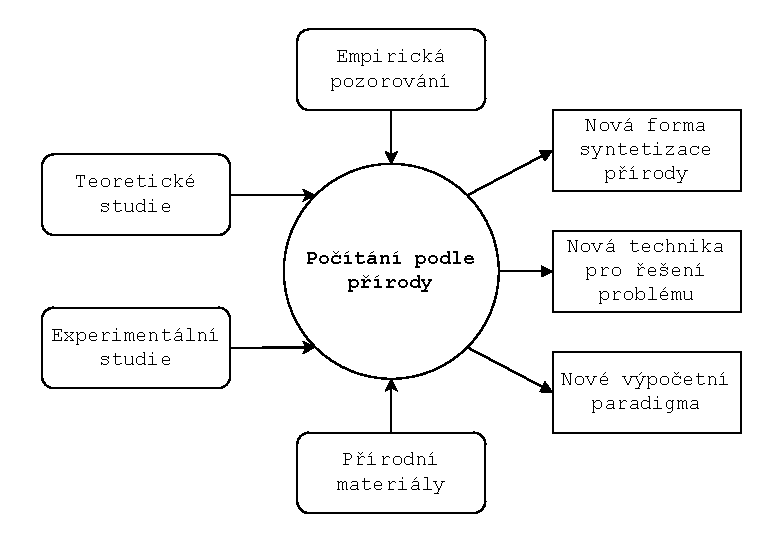
\includegraphics[width=0.75\textwidth]{NaturalComputing-fields.pdf}
    \caption{Výsledkem sjednocení mnoha oblastí výzkumu přírodních procesů jsou nové způsoby řešení problémů~\cite{FundamentalNatural}.}
    \label{fig:natural-computing-fields}
\end{figure}

Počítání podle přírody je možné rozdělit do následujících tří oblastí~\cite{FundamentalNatural}:
\begin{enumerate}
    \item \textbf{Výpočty inspirované přírodou}
        vycházejí z toho, že přírodní procesy dokáží efektivně řešit složité problémy, přičemž tyto přístupy lze rozdělit do dvou hlavních směrů. 
        První vychází z teoretických modelů, s jejichž pomocí lze modelovat přírodní jevy, což pomáhá k lepšímu porozumění fungování různých procesů v přírodě. 
        Druhým směrem je návrh algoritmů, jenž pomáhají řešit složité úlohy, u nichž tradiční přístupy selhávají, přičemž tyto algoritmy využívají určitou úroveň abstrakce nad vybranými přírodními procesy.
        Mezi nejvýznamnější oblasti výpočtů inspirovaných přírodou patří:
        \begin{itemize}
            \item umělé neuronové sítě (\emph{artificial neural networks}) inspirované nervovými systémy,
            \item evoluční algoritmy (\emph{evolutionary algorithms}) vycházející z Darwinovy teorie evoluce,
            \item inteligence roje (\emph{swarm intelligence}) založená na kolektivním chování společenských organismů a
            \item umělé imunitní systémy (\emph{artificial immune systems}) vycházející z principů fungování imunitního systému.
        \end{itemize}
        Příklady výše zmíněných oblastí obsahují například aplikaci umělých neuronových sítí spadá rozpoznávání hlasu, klasifikace objektů či v počítačovém vidění~\cite{ANN-review,ANN-survey}. 
        Evoluční algoritmy je možné uplatnit při řešení různých optimalizačních problémů a inteligence roje je aplikovatelná například při návrhu autonomních robotických systémů nebo při prohledávání stavového prostoru. 
        Umělé imunitní systémy jsou aplikovatelné na komplexní problémy v oblastech od biologie až po robotiku. 
    \item \textbf{Simulace a emulace přírody pomocí výpočetní techniky}
        se zaměřuje na syntézu a studium přírodních fenoménů nebo vzorců či chování a to prostřednictvím simulace, jenž je realizována na výpočetních systémech. 
        Tato oblast poskytuje nástroje pro testování biologických teorií, které by bylo obtížné ověřit za pomoci experimentálních a analytických metod. Existují dva hlavní přístupy:
        \begin{itemize}
            \item Fraktální geometrie v přírodě (\emph{fractal geometry of nature}) poskytuje možnost vizualizovat různé přírodní struktury a procesy, jenž se charakterizují nekonečnou úrovní detailu, nekonečným délkou nebo soběpodobností. 
                Struktura na nichž je viditelná fraktální geometrie se nachází například na kapradinách, horách nebo brokolici a dokonce je patrná na organismech v podobě fraktálové struktury plic, oběhového systému či mozku. 
            \item Umělý život (\emph{artificial life}) je oblast, jež se snaží simulovat organismy v umělých prostředích. Hlavním cílem není řešení konkrétního problému, ale pochopení konceptů přírody včetně vývoje nových forem života. 
        \end{itemize}
        Aplikace fraktální geometrie lze využít při simulaci růstu rostin nebo formování přírodních struktur a umělý život je možno použít pro studii evoluce a chování organismů ve virtuálním prostředí či pro analýzu počítačových virů. 
    \item \textbf{Výpočty s využitím přírodních materiálů} 
        nepracují s křemíkem jako je tomu u~tradičních výpočetních systémů, ale využívají odlišné materiály, jenž umožňují překonat některé limity tradičních počítačů, jelikož poskytují odlišné přístupy k provádění výpočetních operací. 
        Systémy založené na těchto principech nabízejí efektivní řešení problému limitů miniaturizace elektroniky založené na křemíku. 
        Alternativní výpočetní prostředky jsou:
        \begin{itemize}
            \item Molekulární počítání (\emph{Molecular computing}) využívá biologické molekuly, jako je například DNA, k uchování informace, přičemž samotný paralelní výpočet probíhá pomocí manipulace se samotnou molekulou. 
                Výhodou výpočtů založených na molekulách poskytují vysokou rychlost výpočtu, energetickou efektivitu a levné úložiště informací.  
            \item Kvantové počítání (\emph{quantum computing}) využívá principy kvantové mechaniky, kde je informace uchována na mikroskopické úrovni. 
        \end{itemize}
        Výše uvedené prostředky lze využít k efektivnímu řešení některých problémů, kdy molekulární počítání umožnilo efektivně řešit problém Hamiltonovské cesty~\cite{molecular}, zatímco kvantové počítání se ukázalo jako efektivní například při faktorizaci čísel. 
\end{enumerate}
Tato kapitola se dále zaměří na kvantové evoluční počítání, které spojuje kvantový výpočet s principy evolučních algoritmů.

\section{Evoluční algoritmy}
Ačkoliv existuje mnoho variant evolučních algoritmů, všechny vycházejí ze stejné myšlenky, která spočívá v tom, že v prostředí s omezenými zdroji dochází mezi jednotlivci, jejichž schopnost je určena kvalitativní funkcí, k soutěži o~přežití, jejímž výsledkem je přirozený výběr jedinců, jenž zvyšují kvalitu populace. 
Proces spočívá v aplikaci kvalitativní funkce na náhodně vygenerovanou populaci kandidátních řešení, následovaném opakovaným výběrem některých jedinců, na něž je aplikována selekce, rekombinace, mutace až do nalezení dostatečně kvalitního řešení nebo do dosažení nastaveného počtu opakování.  
Evoluční proces lze chápat jako postupnou optimalizaci, která postupně hledá lepší řešení tím, že se přibližuje k optimálnímu stavu~\cite{IntroductionToEvoComputing}. 

Základní elementy evolučního procesu jsou:
\begin{itemize}
    \item variační operátory (rekombinace a mutace), jenž vytvářejí diverzitu v populaci a
    \item selekce, která zvyšuje průměrnou kvalitu řešení v populaci.
\end{itemize}
Evoluční proces je založen na stochastickém chování, respektive během selekce, rekombinace a mutace figuruje prvek náhody~\cite{IntroductionToEvoComputing}. 

Základní schéma evolučního procesu je znázorněno v~algoritmu~\ref{alg:ea-algo}.

\begin{algorithm}[H]
    \caption{Obecné schéma evolučního algoritmu~\cite{IntroductionToEvoComputing}}
    \label{alg:ea-algo}
    \emph{Inicializace} populace náhodně vygenerovanými kandidátními řešeními\;
    \emph{Ohodnocení} každého kandidátního řešení\;
    \While{\emph{není splněna} ukončovací podmínka}{
        \emph{Selekce} rodičů\;
        \emph{Rekombinace} párů rodičů\;
        \emph{Mutace} vzniklých potomků\;
        \emph{Ohodnocení} nových kandidátních řešení\;
        \emph{Selekce} jedinů pro další generaci\;
    }
\end{algorithm}

Podle způsobu reprezentace kandidátských řešení lze evoluční algoritmy rozdělit do následujících kategorií:
\begin{itemize}
    \item evoluční strategie (\emph{evolution strategies\,--\,ES}) pracující s reálnými vektory,
    \item evoluční programování (\emph{evolutionary programming\,--\,EP}) využívají stavy automatů,
    \item genetické programování (\emph{genetic programming\,--\,GP}) využívající stromové struktury a
    \item genetické algoritmy (\emph{genetic algorithms\,--\,GA}) reprezentující kandidátní řešení pomocí binárních řetězců. 
\end{itemize}
Rozdíly mezi výše zmíněnými kategoriemi jsou především historické, protože výběr vhodného typu závisí na povaze řešeného problému, neboť v některých případech je určitý typ reprezentace výhodnější než jiný, pokud lépe odpovídá charakteru problému a usnadňuje reprezentaci kandidátních řešení nebo je přirozenější pro řešený problém~\cite{IntroductionToEvoComputing}. 

Pro definici konkrétního evolučního algoritmu je potřeba specifikovat jeho následující části:

\subsubsection*{Reprezentace}
Prvním krokem je definice reprezentace možných řešení problému, která umožňuje efektivní manipulaci s těmito řešením v rámci algoritmu. 
Možná řešení problému, označovaná jako fenotypy, jsou zakódována do tvarů zvaných jako genotypy, s nimiž algoritmus dokáže pracovat. 
Dochází tak k mapování prostoru fenotypů na prostor genotypů, přičemž ohodnocovací funkce hodnotí fenotypy, ale ohodnocení je přiřazeno genotypům. 
Význam tohoto principu spočívá v tom, že pro algoritmus může být efektivní pracovat například s~binární reprezentací řešení, i když samotný problém má řešení v oblasti celých čísel, vizte obrázek~\ref{fig:fenotyp-to-genotyp}~\cite{IntroductionToEvoComputing,NaturalComputing}. 
\begin{figure}[ht!]
    \centering
    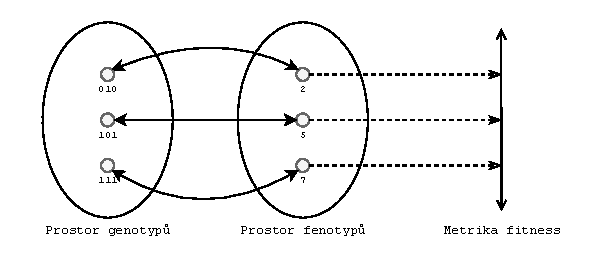
\includegraphics[width=0.75\textwidth]{FenotypToGenotyp.pdf}
    \caption{Mapování z prostoru genotypů na prostor fenotypů, kde každý fenotyp je následně mapován na hodnotu fitness. Obrázek převzat s úpravami z~\cite{NaturalComputing}.}
    \label{fig:fenotyp-to-genotyp}
\end{figure}

V literatuře se v kontextu řešeného problému se fenotyp často ekvivalentně označuje jako kandidátní řešení nebo jedinec. 
Na straně evolučního algoritmu se pro genotyp často používají označení jako chromozom nebo opět jedinec~\cite{IntroductionToEvoComputing}.

\subsubsection*{Inicializace populace}
V evolučních algoritmech je většinou populace inicializována pomocí náhodně generovaných jedinců. 
Pro inicializaci počáteční populace je možné využít i heuristiku, která, pokud je výpočetně přijatelná, vytvoří populaci s vyššími hodnotami fitness. 

\subsubsection*{Ohodnocovací funkce (fitness funkce)}
Hlavním účelem ohodnocovací funkce je řízení evolučního procesu tím, že hodnotí, jak dobře populace splňuje určené požadavky. 
Jedná se o funkci, jenž přiřazuje míru kvality genotypům prostřednictvím ohodnocení odpovídajících fenotypů. 
Ohodnocovací funkce je běžně označována jako fitness funkce. 
V případě optimalizačního problému, je často používán pojem objektivní funkce, který vyjadřuje specifické požadavky úlohy (například maximalizaci nebo minimalizaci určité hodnoty).
Ohodnocovací (fitness) funkce může být identická s~objektivní funkcí nebo se může jednat o její transformaci:
\begin{equation*}
    F\left( x \right) = g\left( f \left( x \right)\right),
\end{equation*}
kde $f(x)$ je objektivní funkce a $g(x)$ je transformační funkce, jež upravuje hodnotu objektivní funkce pro potřeby selekce a hodnocení v evolučním algoritmu~\cite{IntroductionToEvoComputing,NaturalComputing}. 

\subsubsection*{Populace}
Hlavní rolí populace v evolučních algoritmech je uchování možných řešení problému. 
Populace je chápána jako multimnožina genotypů, která se v průběhu evoluce mění, přičemž genotypy jsou pouze statické objekty, vizte obrázek~\ref{fig:population}. 
\begin{figure}[ht!]
    \centering
    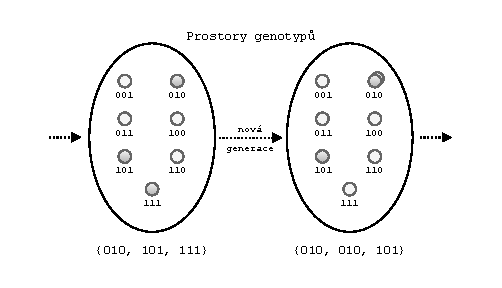
\includegraphics[width=0.67\textwidth]{population.pdf}
    \caption{Populace je multimnožina genotypů, kde se mohou stejné genotypy vyskytovat vícekrát, přičemž složení populace se může měnit s každou novou generací pomocí selekce, rekombinace a mutace.}
    \label{fig:population}
\end{figure}
Velikost populace je obvykle konstantní, což vytváří podmínky pro přirozený výběr jedinců vlivem omezených zdrojů a~nutnosti soutěžení o přežití.

\subsubsection*{Selekce rodičů}
Rodičem se stává jedinec, jenž byl vybrán k tomu, aby podstoupil proces změny, ať už rekombinací nebo mutací, čímž vytváří potomky. 
        Obvykle se rodičem stává kvalitní jedinec, avšak vzhledem k tomu, že proces selekce bývá stochastický, může se rodičem stát i málo kvalitní jedinec, což poskytuje vyšší diverzitu, jež pomáhá předcházet uvíznutí v lokálním optimu~\cite{IntroductionToEvoComputing}. 
\subsubsection*{Variační operátory}
Cílem variačních operátorů je vytvořit z existujících jedinců nové. 
V kontextu fenotypového prostoru dochází ke generování nových kandidátních řešení. 
Dle arity se variační operátory dělí na následující dva typy:
\begin{itemize}
    \item \textbf{Mutace} je unární operátor, jenž je aplikován na rodiče a jehož výsledkem je potomek. 
        Tento potomek vznikl na základě sérií náhodných voleb, která vedou k~úpravám genotypu, pokud jsou splněny určité podmínky, vizte obrázek~\ref{fig:mutation}~\cite{IntroductionToEvoComputing,NaturalComputing}. 
        \begin{figure}[ht!]
            \centering
            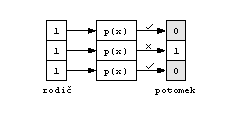
\includegraphics[width=0.6\textwidth]{Mutation.pdf}
            \caption{Proces mutace rodiče, kde funkce $p(x)$ určuje pravděpodobnostní rozhodnutí, zda bude provedena mutace konkrétní části genomu. Na základě této série náhodných rozhodnutí vznikne potomek.}
            \label{fig:mutation}
        \end{figure}
    \item \textbf{Rekombinace}, někdy označovaná jako křížení, je n-ární operátor, jenž kombinuje informace z vícero rodičů. 
        Standardně se v přírodě objevuje pouze binární rekombinace, ale v evolučním počítání je možné uvažovat i křížení s větší aritou. 
        Podobně jako mutace je i rekombinace založena na stochastickém principu, což znamená, že výběr částí, které budou z každého rodiče kombinovány, je založen na náhodné volbě. 
        Pro příklad jednoduché rekombinace vizte obrázek~\ref{fig:crossover}~\cite{IntroductionToEvoComputing}. 
        \begin{figure}[ht!]
            \centering
            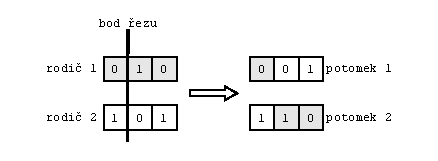
\includegraphics[width=0.8\textwidth]{Crossover.pdf}
            \caption{Ilustrace jednobodové binární rekombinace, kde se na základě náhodně vybraného bodu řezu kombinují informace z rodičovských genotypů do nově vzniklých potomků. Obrázek převzat s úpravami z~\cite{NaturalComputing}}
            \label{fig:crossover}
        \end{figure}
\end{itemize}
Mutace v evolučních algoritmech zajišťuje neustálý vývoj evolučního procesu, jelikož v~každé iteraci s určitou pravděpodobností umožňuje objevování nových vlastností. 
Na rozdíl od rekombinace, která pokud je jediným zdrojem diverzity, přestává vytvářet nová řešení v~případě, že populace konvergovala k jednomu genotypu~\cite{NaturalComputing}. 

\subsubsection*{Selekce přeživších}
Podobně jako u selekce rodičů, i u selekce přeživších jsou jedinci vybíráni na základě jejich kvality ale až posléze, co jsou vytvořeni potomci z vybraných rodičů. 
Jelikož velikost populace je ve většině případů konstantní, je nutné rozhodnout o tom, kteří jedinci budou figurovat v další generaci. 
Toho rozhodnutí může záviset nejen na hodnotě fitness, ale může být zohledněn i věk jedinců, což značí, že selekce jedinců do nové generace je ve většině případů deterministická. 

Příkladem jedné z nejběžnějších strategií pro selekci je sjednocení množiny rodičů a~potomků, jejich seřazení na základě hodnoty fitness a výběr nejlepších jedinců pro novou generaci. 

\subsubsection*{Ukončovací podmínka}
Evoluční proces je ukončen splněním ukončovací podmínky, kterou lze rozdělit do dvou hlavních případů. 
V prvním případě je evoluční algoritmus ukončen po nalezení jedince, jehož hodnota fitness se shoduje s dříve známou optimální hodnotou. 
Ve druhém případě, kdy je řešený problém zjednodušen nebo obsahuje šum, je akceptováno řešení, které se dostatečně blíží optimálnímu řešení v rámci požadované přesnosti. 
Jelikož jsou evoluční algoritmy stochastické, není vždy zaručeno dosažení optimálního řešení, což může vést k~nekončícímu evolučnímu procesu.
Proto je nutné zavedení následujících podmínek, jejichž splnění zajistí ukončení evoluce:
\begin{enumerate}
    \item Uplynutí maximálního povoleného procesorového času.
    \item Dosažení maximálního počtu vyhodnocení fitness funkce. 
    \item Po určitou dobou nedochází ke zlepšení fitness nad určitou prahovou hodnotu.
    \item Diverzita populace klesne pod vybraný bod.
\end{enumerate}
Pokud není známo optimální řešení problému, stačí pro ukončení evolučního algoritmu použít jakoukoliv z výše uvedených podmínek. 

\section{Základy kvantové fyziky}
Tato sekce poskytne stručný popis základních oblastní fyziky a jejich vzájemných souvislostí. 
Následně se zaměří na podrobnější popis vybrané oblasti, konkrétně kvantové mechaniky, jejíž popis je nutný pro hlubší pochopení kapitoly~\ref{chapt:qiea} věnované algoritmům inspirovaných z této oblasti fyziky.

Obrázek~\ref{fig:mechanics} vyobrazuje základní dělení moderní fyziky na základní části (nepřerušované obdélníky) společně s~jejich vzájemnými vztahy. 
Nepřerušované šipky ukazují nové fyzikální teorie, které vznikly za pomoci úpravy té starší a to buď odstraněním některých z jejich předpokladů nebo přidáním nových principů.
Přerušované obdélníky značí nejznámější fyzikálně inspirované algoritmy, přičemž přerušované šipky znázorňují z jakých fyzikálních konceptů tyto algoritmy vycházejí~\cite{NaturalComputing}.

\begin{figure}[ht!]
    \centering
    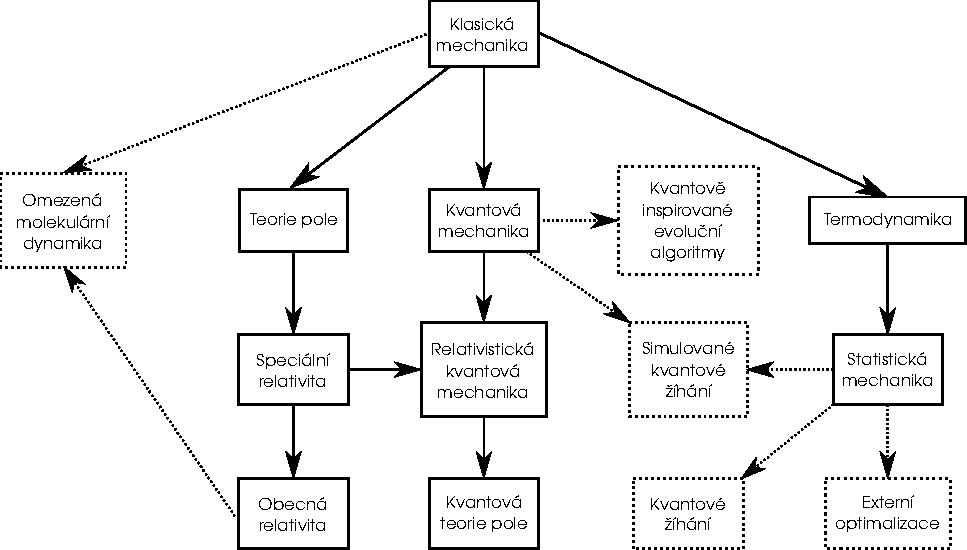
\includegraphics[width=\textwidth]{mechanics.pdf}
    \caption{Vazby mezi fyzikálními principy a algoritmy. Diagram byl převzat s úpravami z~\cite{NaturalComputing}.}
    \label{fig:mechanics}
\end{figure}

Jednotlivé základní oblasti fyziky společně s jejich stručným popisem je následující~\cite{NaturalComputing}:
\begin{itemize}
    \item \textbf{Klasická mechanika (\emph{Classical Mechanics}):} 
    Podle Galileiho a Newtona působí na tělesa síly, které jsou vnímány jako síly působící okamžitě a na dálku. 
    Euler, Laplace, Lagrange, Hamilton a další vytvořili alternativní formulace pomocí skalární energie, které jsou s původní formulací ekvivalentní. 
    \item \textbf{Teorie pole (\emph{Filed Theory}):} 
    Koncept formulovaný Maxwellem a dalšími popisující, jak mohou objekty generovat skalární potencionální pole, které vytváří odpovídající vektorové pole (například gravitační nebo elektromagnetické), jež následně ovlivňuje ostatní objekty. 
    Tato pole můžou přenášet energii prostorem ve formě vln, což omezuje rychlost šíření signálů, čímž odstraňuje okamžité působení síly na dálku. 
    Tato teorie mimo jiné ukazuje, že se světlo šíří ve vakuu konstantní konečnou rychlostí. 
    \item \textbf{Speciální teorie relativity (\emph{Special Theory of Relativity}):} 
    Dílo Einsteina vycházející z toho, že fyzikální zákony jsou ve všech inerciálních vztažných soustavách stejné společně s faktem, že rychlost světla ve vakuu je vždy konstantní.
    \item \textbf{Obecná teorie relativity (\emph{General Theory of Relativity}):} 
    Rozšířená speciální teorie relativity samotným Einsteinem, která zavádí princip ekvivalence mezi rovnoměrným gravitačním polem a zrychlením. 
    \item \textbf{Kvantová mechanika (\emph{Quantum Mechanics}):} 
    Koncept podle Plancka, Bohra, Schrö\-din\-ge\-ra, Heisenberga, Pauliho, Einsteina a dalších zavádějící mimo jiné pojem kvantování, který nahrazuje pozorovatelné fyzikální veličiny, jako je například poloha či energie, operátory v Hilbertově prostoru vlnových funkcí.
    \item \textbf{Relativistická kvantová mechanika (\emph{Relativistic Quantum Mechanics}):} 
    Teorie, kde Schrödingerova rovnice pro elektron byla upravena do relativisticky invariantní podoby Diracem tak, že vlnové vektory mají přidané stupně volnosti, které přesně modelují spin elektronu. 
    Tato teorie předpověděla existenci antihmoty, respektive pozitronu. 
    \item \textbf{Kvantová teorie pole (\emph{Quantum Field Theory}):} 
    Dílo Feynmana a dalších, které za pomoci Diracovi práce rozšiřuje relativistickou kvantovou mechaniku tím, že kvantizuje samotné pole včetně vlnové funkce. 
    Tento postup umožňuje interpretovat interakci sil prostřednictvím výměny částic. Praktickým příkladem je Feynmanova kvantová elektrodynamika. 
    \item \textbf{Termodynamika (\emph{Thermodynamics}):} 
    Teorie formulovaná Carnotem, Boltzmannem a dalšími, která se zabývá makroskopickými fyzikálními veličinami, jako je například tlak a teplota, u systému složených z mikroskopických částic. 
    Popisuje mimo jiné koncept termodynamické rovnováhy, termodynamických procesů a entropie. 
    \item \textbf{Statistická mechanika (\emph{Statistical Mechanics}):} 
    Moderní pohled na termodynamiku, který popisuje makroskopické veličiny pomocí statistického chování částic.
\end{itemize}

Následující sekce se podrobněji zaměří na odnož klasické mechaniky, konkrétně na kvantovou mechaniku, která slouží jako inspirace pro kvantově inspirované algoritmy.

\section{Kvantová mechanika}
Model chování přírodních systémů pozorovaných na velmi krátkých časových a délkových měřítkách popisuje kvantová mechanika, která je rozšířením klasické mechaniky. 
Kvantový systém se může skládat z jedné nebo více částic, jako je například volný elektron či foton. 

Použitím kvantizace dochází k nahrazení proměnných reprezentujících pozorovatelné fyzikální veličiny, jako jsou poloha, hybnost či energie, lineárními operátory ve vhodném vektorovém prostoru. 
Tento vektorový prostor nese název Hilbertův prostor (\emph{Hilbert space}) a je definován jako kompletní vnitřní součinový prostor nad komplexními čísly. 
Jeho prvky jsou funkce časových a prostorových souřadnic, které reprezentují kvantové stavy systému. 
Kvantový stav systému $\psi$ je někdy rovněž označován jako stavový vektor, vlnová funkce nebo vlnový vektor. 
Na prvky Hilbertova prostoru působí lineární operátory (\emph{observables}), které reprezentují pozorovatelné fyzikální veličiny. 
Vlastní hodnoty těchto operátorů odpovídají možným výsledkům pozorování daných fyzikálních veličin~\cite{NaturalComputing}.

Následující části stručně popisují klíčové koncepty kvantové mechaniky:

\subsubsection*{Pozorování v kvantové mechanice}
Pozorování kvantového systému vede k určení hodnoty pozorovatelné veličiny, přičemž pravděpodobnost pozorování konkrétní hodnoty odpovídá kvadrátu absolutní hodnoty vlnové funkce $\psi$.
Kvadrát absolutní hodnoty $\left| \psi \right|^2$ představuje hustotu pravděpodobnosti, která udává pravděpodobnost nalezení částice na dané pozici v daném čase v prostoru. 
    
Časový vývoj vlnové funkce a tedy i hustoty pravděpodobnosti v každém bodě prostoru je popsán lineární Schrödingerovou rovnicí. 
V čase se kvantový stav vyvíjí deterministicky podle této rovnice, což způsobuje rozptyl hustoty pravděpodobnosti v prostoru. 
Kvantový stav se před provedením pozorování nachází v superpozici, tedy v lineární kombinaci všech možných vlastních stavů (\emph{eigenstates}) operátoru odpovídajícího pozorované veličině. 
    
S postupem času se hustota pravděpodobnosti stále více rozprostírá, což vede ke zvyšování neurčitosti polohy částice. 
Tento proces pokračuje, dokud není provedeno pozorování, při kterém vlnová funkce nelineárně kolabuje do jednoho z vlastních stavů měřené veličiny. 
Pravděpodobnost nalezení systému v konkrétním vlastním stavu je dána hodnotou $\left| \psi \right|^2$ v~tomto stavu, přičemž nalezení částice je nejvyšší v oblastech, kde je hodnota $\left| \psi \right|$ největší, a nulová tam, kde $\left| \psi \right| = 0$.
    
Normalizované vlnové funkce splňují podmínku
\[
    \int_{\mathbb{R}^3} \left|\psi\,(x)\right|^2 dx = 1.
\]
Tato rovnost vyjadřuje, že celková pravděpodobnost nalezení částice v celém prostoru musí být rovna 1.
Z toho plyne, že kvantové stavy leží v jednotkové kouli Hilbertova prostoru, tedy v množině všech vektorů s normou 1 a operátory, které na ně působí, musí být unitární, aby tuto normu zachovávaly~\cite{NaturalComputing}.

\subsubsection*{Kvantové provázání}
Pojem kvantové provázání (\emph{entanglement}) je jeden z nejdůležitějších rozdílů mezi klasickou a kvantovou fyzikou. 
V kvantovém systému složeného z více částic existuje pouze jedna vlnová funkce, kterou nelze rozdělit na nezávislé vlnové funkce jednotlivých částic. 
Podle Schrödingerovy rovnice se tato vlnová funkce vyvíjí v čase do té doby, dokud není provedeno pozorování.
Kolaps vlnové funkce celého systému nastává při jeho pozorování a okamžitě ovlivňuje stav všech provázaných částic, které následně přecházejí do jednoho z vlastních stavů měřené veličiny.

V klasickém systému složeném z $m$ částic, kde každá může nabývat $n$ různých stavů, roste dimenze prostoru lineárně jako $n \times m$, neboť prostor je dán přímým součtem.
V~kvantovém systému je však správným prostorem tenzorový součin, což způsobuje, že jeho dimenze roste exponenciálně jako $n^m$~\cite{NaturalComputing,QuantumComputing-QuantumInformation}.

\subsubsection*{Dekoherence}
V případě, že dojde ke kontaktu makroskopického prostředí (například měřící zařízení) s~kvantovým systémem, dochází k nevratnému úniku kvantových vlastností do okolí v termodynamicky nevratném procesu. 
Dekoherence se projevuje tím, že složky kombinované vlnové funkce systému a prostředí přestanou efektivně interferovat.
Na makroskopické úrovni tento proces vede k rozpadu superpozic stavů, což se jeví jako zdánlivý kolaps vlnové funkce systému~\cite{NaturalComputing}.

\subsubsection*{Nekomutující operátory}
Pokud jakékoli dva operátory $A$ a $B$ komutují, platí pro ně vztah $\left[A, B \right] = A \times B - B \times A = 0$\,\,\footnote{Analogie k Poissonovým závorkám v klasické mechanice.}. 
V kvantové mechanice však operátory obecně nekomutují. 
Příkladem nekomutujících operátorů jsou operátory polohy a hybnosti, jejichž vzájemná nekomutativita vede k Heisenbergově principu neurčitosti.
Tento princip říká, že není možné současně měřit hodnoty obou veličin s požadovanou přesností, respektive měření hodnoty jedné veličiny narušuje odpovídajícím způsobem druhou veličinu~\cite{NaturalComputing,QuantumMeasurement}.

\subsubsection*{Kvantové tunelování}
Kvantové tunelování je jev, při kterém může být částice s~konečnou, nenulovou pravděpodobností pozorována i za bariérou, přestože klasicky by jí neměla být schopna překonat. 
Očekávaný čas tunelování závisí nejen na šířce bariéry, ale i na její výšce, přičemž čím širší je bariéra, tím nižší je pravděpodobnost, že částice projde touto bariérou. 
Tento efekt je důsledkem vlnové povahy částice, protože její vlnová funkce je rozprostřena v prostoru, a~tudíž je nenulová i na opačné straně bariéry~\cite{NaturalComputing}. 

\section{Kvantové evoluční počítání}
Hlavní rozdíl mezi kvantovými a klasickými výpočetními systémy spočívá v jejich výpočetních schopnostech.
Kvantové systémy využívají principy superpozice a provázání, což jim umožňuje efektivněji řešit některé problémy, které jsou pro klasické počítače výpočetně náročné. 

Existují dva hlavní přístupy pro kvantové počítače:
\begin{itemize}
    \item \textbf{Digitální kvantové počítače:} Oproti klasickým počítačům místo bitů využívají qubity.
    \item \textbf{Adiabatické kvantové počítače:} Hledají optimální řešení problémů prostřednictvím postupné evoluce kvantového systému.
\end{itemize}

Jelikož kvantové výpočty vykazují výhody při optimalizaci, vedly k návrhu kvantově inspirovaných evolučních algoritmů, které jsou zařazeny do kvantově evolučního počítání, viz obrázek~\ref{fig:natural-computing}.
Z tohoto důvodu bude těmto kvantovým počítačům věnována tato sekce~\cite{NaturalComputing}.

\begin{figure}[ht!]
    \centering
    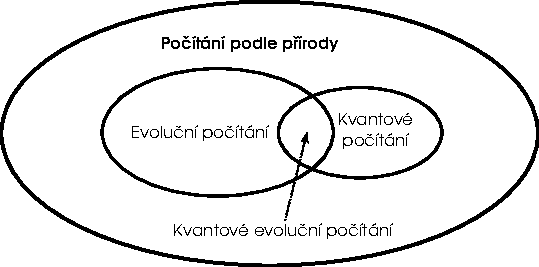
\includegraphics[width=0.65\textwidth]{NaturalComputing.pdf}
    \caption{Kvantové evoluční počítání je kombinací kvantových a evolučních výpočtů, přičemž obě tyto oblasti spadají do výpočtů inspirovaných přírodou. Obrázek byl převzat s~úpravami z~\cite{QuantumComputing-QuantumInformation}.}
    \label{fig:natural-computing}
\end{figure}

\subsection{Kvantový bit}
Superpozice v kontextu klasické fyziky značí situaci, kdy součtem dvou fyzikálních veličin vznikla odlišná fyzikální veličina. 
Případem aplikace této superpozice je výpočet celkové velikosti a směru veličiny, jako je například síla či elektrické pole.
Na rozdíl od klasické fyziky v kvantové mechanice superpozice označuje stav, kdy může být systém současně ve více stavech. 
Tento systém zůstává ve stavu superpozice do té doby, dokud není provedeno jeho pozorování, kdy se superpozice zhroutí a systém bude v jedné konkrétní hodnotě~\cite{QuantumComputing-Curious}. 

Kvantový bit nebo-li qubit se na rozdíl od klasického bitu, který může nabývat pouze hodnot 0 nebo 1, nachází v superpozici těchto stavů. 
Avšak při měření qubitu dojde ke kolapsu jeho superpozice do jednoho ze stavů klasického bitu~\cite{QuantumComputing-Curious}.  

Ve standardním zápisu\,\footnote{Standardně se využívá Diracova nebo \uv{bra-ket} notace.} je kvantový stav qubitu $| \psi \rangle$ vyjádřen jako superpozice stavů $| 0 \rangle$ a $| 1 \rangle$:
\begin{equation}\label{eq:psi=a0+b1}
    | \psi \rangle = \alpha | 0 \rangle + \beta | 1 \rangle, 
\end{equation}
kde koeficienty (amplitudy) $\alpha, \beta \in \mathbb{C}$ umožňují matematicky reprezentovat všechny možné superpozice. 
Tyto koeficienty musí splňovat podmínku normalizace 
\begin{equation}\label{eq:a2+b2=1}
    \left| \alpha \right|^2 + \left| \beta \right|^2 = 1,   
\end{equation}
kde $\left| \alpha \right|^2$, respektive $\left| \beta \right|^2$, udává pravděpodobnost nalezení částice ve stavu $| 0 \rangle$, respektive $| 1 \rangle$, po provedeném měření. 
Podmínka normalizace zajišťuje, že superpozice zkolabuje s~jistotou do jednoho ze stavů $| 0 \rangle$ nebo $| 1 \rangle$~\cite{NaturalComputing,QuantumComputing-Curious}.

Rovnici~\ref{eq:psi=a0+b1} lze díky platnosti rovnosti~\ref{eq:a2+b2=1} přepsat do podoby:
\begin{equation*}
    | \psi \rangle = \cos{\frac{\theta}{2}} | 0 \rangle +  e^{i\phi} \sin{\frac{\theta}{2}} | 1 \rangle,
\end{equation*}
kde hodnoty $\theta$ a $\phi$ určují pozici qubitu na povrchu Blochovy sféry, viz obrázek~\ref{fig:bloch-sphere}. 
Tato sféra umožňuje vizualizaci stavu pouze jednoho qubitu. 
Pro více qubitů již nelze využít tuto geometrickou reprezentaci~\cite{QuantumComputing-Curious,QuantumComputing-QuantumInformation}. 

\begin{figure}[ht!]
    \centering
    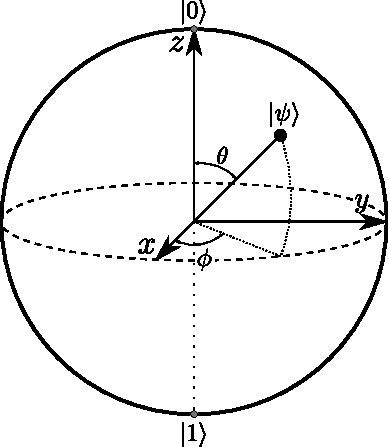
\includegraphics[width=0.45\textwidth]{bloch-sphere.pdf}
    \caption{Blochova sféra reprezentující qubit. Obrázek byl převzat s úpravami z~\cite{QuantumComputing-QuantumInformation}.}
    \label{fig:bloch-sphere}
\end{figure}

\subsection{Kvantová informace}
Princip kvantové provázanosti určuje hlavní rozdíl mezi kvantovým a klasickým bitem, neboť udává silné korelace mezi qubity, což umožňuje pracovat s mnoha stavy současně. 
Tento jev, známý jako kvantový paralelismus, poskytuje kvantovým systémům výpočetní výhodu oproti klasickým systémům, protože umožňuje existenci stavu v podobě superpozice mnoha klasických stavů~\cite{NaturalComputing}.

Vlastnosti kvantové informace způsobující problémy při provádění výpočtů jsou~\cite{NaturalComputing}:
\begin{itemize}
    \item \textbf{Princip neurčitosti:} V případě nekomutujících pozorovaných veličin ovlivní měření jedné veličiny výsledek měření jiné veličiny. 
    \item \textbf{Princip nemožnosti klonování:} Kvantová informace nemůže být dokonale zkopírována, jinak by byl narušen princip neurčitosti. 
    \item \textbf{Princip provázanosti: } Kvantová informace je díky své provázanosti rozložena mezi více částí systému, což ji typicky znemožňuje rozdělit na části (jednotlivé qubity). Tento princip je hlavním důvodem, proč nelze efektivně simulovat kvantové systémy na těch klasických. 
    \item \textbf{Dekoherence: } Při interakci informací kvantového systému s informacemi z okolního prostředí dochází k jejich vzájemnému provázání, což snižuje schopnost obnovit původní kvantovou informaci, neboť většina provázaných informací pochází z okolního prostředí. 
\end{itemize}

\subsection{Digitální kvantové počítače}
Digitální kvantové počítače pracují s qubity a manipulují s nimi pomocí kvantových bran (ekvivalent bitových operátorů).
V průběhu výpočtu jsou tyto brány aplikovány na systém qubitů a měření qubitů je provedeno až na konci samotného výpočtu. 
Paul Benioff uvažoval Turingův stroj pracující s ekvivalentem qubitů a později Richard Feynman dokázal, že klasické počítačové systémy nejsou schopny efektně simulovat kvantové systémy zejména kvantové provázání, protože by jejich simulace vyžadovala exponenciální časovou a paměťovou složitost, respektive $\mathcal{O}\left( 2^n \right)$~\cite{NaturalComputing,QuantumComuting-Introduction}. 

Kvantové počítače prokazatelně umožňují oproti těm klasickým řešit některé druhy problémů efektivněji. 
Příklad algoritmu, který je schopný řešit problém v kvantovém počítači účiněji je: 
\begin{itemize}
    \item \textbf{Shorův algoritmus:} Umožňuje faktorizaci velkých čísel v časové složitosti $\mathcal{O}\left( n^2 \right)$ místo $\mathcal{O}\left(e^{\sqrt[3]{n}} \right)$, jako je tomu u nejlepšího známého algoritmu na klasických systémech.
    \item \textbf{Groverův algoritmus:} Zrychluje vyhledávání v nestrukturovaných databázích klasických systémů z časové složitosti $\mathcal{O}\left( n \right)$ na $\mathcal{O}\left( \sqrt{n} \right)$. 
\end{itemize}
Mimo jiné umožňují kvantové počítače simulovat sami sebe, přičemž však stále není známo zda dokážou řešit NP těžké problémy v polynomiálním čase~\footnote{Obecně se věří, že nedokážou řešit NP těžké problémy v polynomiálním čase.}~\cite{NaturalComputing}. 

\subsection{Adiabatické kvantové počítače}
Oproti digitálním kvantovým počítačům se adiabatické kvantové počítače neskládají z qubitů. 
Místo toho využívají postupnou evoluci kvantového systému v čase. 
Přístup je podobný analogovým počítačům, kde je vytvořen fyzikální systém odpovídající řešenému problému a jeho stav je ponechán, aby se vyvíjel v čase. 
Jejich výpočetní síla je ekvivalentní s kvantovými počítači založenými na qubitech, což znamená, že dokážou řešit stejné problémy se srovnatelnou polynomiální složitostí~\cite{NaturalComputing}.

Adiabatické kvantové počítače splňují kvantový adiabatický teorém, jehož hlavní myšlenkou je, že pokud jsou na systém aplikovány vnější jevy dostatečně pomalu, zůstává ve svém relativním vlastním stavu. 
Pokud jsou však změny vnějších jevů aplikovány na systém příliš rychle, stav systému se nezmění, jelikož nemá dostatek času na to se přizpůsobit a~skončí v superpozici stavů~\cite{NaturalComputing}. 

Princip evoluce v adiabatických kvantových počítačích je hlavní myšlenkou adiabatického kvantového počítání (\emph{Adiabatic Quantum Computing\,--\,AQC}). 
To svým principem připomínají tepelné žíhání kovů, proto se rovněž označuje jako kvantové žíhání (\emph{Quantum Annealing\,--\,QA})~\cite{NaturalComputing}. 
